\documentclass[aspectratio=169, xcolor={table,dvipsnames}]{beamer}

% ============================================
% PACKAGES
% ============================================
\usepackage[utf8]{inputenc}
\usepackage[T1]{fontenc}
\usepackage{helvet} % Cleaner font
\usepackage{tikz}
\usepackage{pgfplots}
\usepackage{booktabs} % For nicer tables
\usepackage{fontawesome5} % For icons
\usepackage{listings}
\usepackage{multicol}

% TikZ Libraries
\usetikzlibrary{shapes.geometric, arrows.meta, positioning, calc, shadows, fit, backgrounds}
\pgfplotsset{compat=1.18}

% ============================================
% THEME & COLORS
% ============================================
\usetheme{Madrid}
\usecolortheme{whale}
\setbeamertemplate{navigation symbols}{} % Remove nav symbols
\setbeamertemplate{footline}[frame number]

% Custom Colors based on the presentation style
\definecolor{primary}{RGB}{56, 189, 248}    % Light Blue
\definecolor{secondary}{RGB}{99, 102, 241}  % Indigo
\definecolor{accent}{RGB}{244, 63, 94}      % Pink/Red
\definecolor{success}{RGB}{16, 185, 129}    % Green
\definecolor{warning}{RGB}{245, 158, 11}    % Orange
\definecolor{darkbg}{RGB}{30, 41, 59}       % Dark Slate

% ============================================
% META INFO
% ============================================
\title[School Club Activity]{\textbf{School Club Activity Showcase}}
\subtitle{Software Engineering 1 -- Final Project Presentation}
\author[Team 9]{
    \textbf{Team 9:}\\
    Francesco Bolner \quad Georgi Bozhkov \quad Samuele Fumagalli\\
    Ayoub Merdan \quad Martin Ushilov
}
\institute{Software Engineering Course}
\date{December 2025}

\begin{document}

% ============================================
% SLIDE 1: TITLE
% ============================================
\begin{frame}
    \titlepage
\end{frame}

% ============================================
% SLIDE 2: AGENDA
% ============================================
\begin{frame}{Agenda}
    \begin{multicols}{2}
        \tableofcontents
    \end{multicols}
\end{frame}

% ============================================
% SLIDE 3: OVERVIEW
% ============================================
\section{Project Overview}
\begin{frame}{Project Overview}
    \begin{columns}[T]
        \column{0.5\textwidth}
        \textbf{\large What is School Club Activity?}
        \vspace{0.3cm}
        
        A \textbf{full-stack web application} designed to manage school club activities, enabling students to:
        \begin{itemize}
            \item \faSearch\ Browse and discover clubs
            \item \faUserPlus\ Request membership
            \item \faClipboardList\ View and track events
            \item \faStar\ Leave reviews and ratings
            \item \faBell\ Receive real-time notifications
        \end{itemize}
        
        \vspace{0.2cm}
        \textbf{Target Users:} School pupils with valid School ID.

        \column{0.5\textwidth}
        % Mindmap Diagram
        \begin{center}
        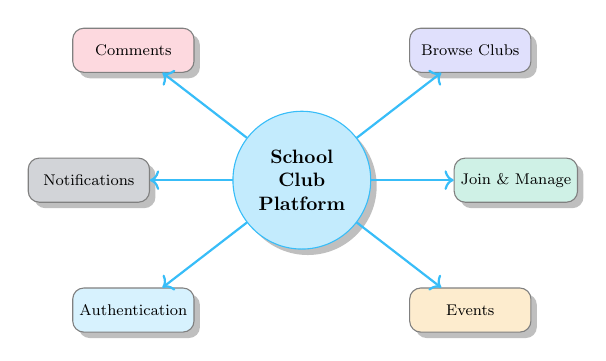
\begin{tikzpicture}[scale=0.7, transform shape,
            node distance=1.5cm,
            center/.style={circle, fill=primary!30, draw=primary, minimum size=2.5cm, font=\bfseries, align=center, drop shadow},
            feature/.style={rectangle, rounded corners, draw=gray, fill=white, minimum height=0.8cm, minimum width=2.2cm, font=\footnotesize, drop shadow}
        ]
            \node[center] (core) {School\\Club\\Platform};
            
            \node[feature, fill=secondary!20, above right=of core] (browse) {Browse Clubs};
            \node[feature, fill=success!20, right=of core] (join) {Join \& Manage};
            \node[feature, fill=warning!20, below right=of core] (events) {Events};
            \node[feature, fill=accent!20, above left=of core] (comments) {Comments};
            \node[feature, fill=darkbg!20, left=of core] (notif) {Notifications};
            \node[feature, fill=primary!20, below left=of core] (auth) {Authentication};

            \foreach \x in {browse, join, events, comments, notif, auth}
                \draw[->, thick, primary] (core) -- (\x);
        \end{tikzpicture}
        \end{center}
    \end{columns}
\end{frame}

% ============================================
% SLIDE 4: REQUIREMENTS
% ============================================
\section{Main Requirements}
\begin{frame}{Functional Requirements}
    \begin{columns}[T]
        \column{0.5\textwidth}
        \textbf{\faUser\ User Management}
        \begin{itemize}
            \item Secure login/signup with bcrypt hashing
            \item Session-based authentication
            \item Role-based access control (RBAC)
        \end{itemize}
        
        \vspace{0.2cm}
        \textbf{\faUsers\ Club Management}
        \begin{itemize}
            \item Create new clubs with member limits
            \item Update descriptions (HTML supported)
            \item Delete clubs (cascading cleanup)
            \item Custom banners and colors
        \end{itemize}
        
        \column{0.5\textwidth}
        \textbf{\faCalendarCheck\ Event Management}
        \begin{itemize}
            \item Create events with date ranges
            \item Approval workflow (pending/accepted)
            \item ICS calendar export
        \end{itemize}
        
        \vspace{0.2cm}
        \textbf{\faComment\ Social Features}
        \begin{itemize}
            \item Comment on clubs with star ratings
            \item Real-time notifications
            \item Member management (promote/expel)
        \end{itemize}
    \end{columns}
\end{frame}

% ============================================
% SLIDE 5: ROLES
% ============================================
\begin{frame}{User Roles Hierarchy}
    \begin{center}
        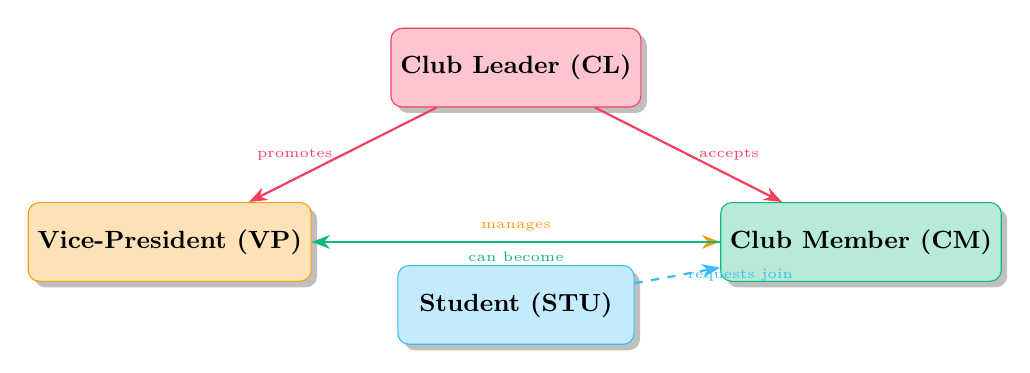
\begin{tikzpicture}[
            node distance=1.2cm and 1cm,
            role/.style={rectangle, rounded corners, draw, minimum width=3cm, minimum height=1cm, font=\small\bfseries, align=center, drop shadow},
            arrow/.style={-{Stealth}, thick}
        ]
            % Nodes
            \node[role, fill=accent!30, draw=accent] (cl) {Club Leader (CL)};
            \node[role, fill=warning!30, draw=warning, below left=of cl] (vp) {Vice-President (VP)};
            \node[role, fill=success!30, draw=success, below right=of cl] (cm) {Club Member (CM)};
            \node[role, fill=primary!30, draw=primary, below=2cm of cl] (stu) {Student (STU)};
            
            % Arrows
            \draw[arrow, accent] (cl) -- node[left, font=\tiny] {promotes} (vp);
            \draw[arrow, accent] (cl) -- node[right, font=\tiny] {accepts} (cm);
            \draw[arrow, warning] (vp) -- node[above, font=\tiny] {manages} (cm);
            \draw[arrow, success] (cm) -- node[below, font=\tiny, sloped] {can become} (vp);
            \draw[arrow, primary, dashed] (stu) -- node[right, font=\tiny] {requests join} (cm);
        \end{tikzpicture}
    \end{center}
\end{frame}

% ============================================
% SLIDE 6: NFR
% ============================================
\begin{frame}{Non-Functional Requirements}
\small
\begin{columns}[T]
    \column{0.33\textwidth}
    \begin{block}{\faTachometerAlt\ Performance}
        \begin{itemize}
            \item Fast page loads (Home / Clubs / Events)
            \item Handles many simultaneous users
            \item Responsive actions: login, register, enroll/unenroll, join club/event
        \end{itemize}
    \end{block}

    \column{0.33\textwidth}
    \begin{block}{\faShieldAlt\ Security}
        \begin{itemize}
            \item Role-based access for protected actions
            \item Only authorized roles can edit clubs, approve events, change roles
            \item Session timeout requires re-login for protected actions
        \end{itemize}
    \end{block}

    \column{0.33\textwidth}
    \begin{block}{Compatibility}
        \begin{itemize}
            \item Logs include timestamps and user identifiers
            \item Works on latest Chrome, Safari, Edge
            \item Phone support
        \end{itemize}
    \end{block}
\end{columns}
\end{frame}

% ============================================
% SLIDE 8: DEVELOPMENT
% ============================================
\section{Development Methodology}
\begin{frame}{Development Methodology}
\begin{center}
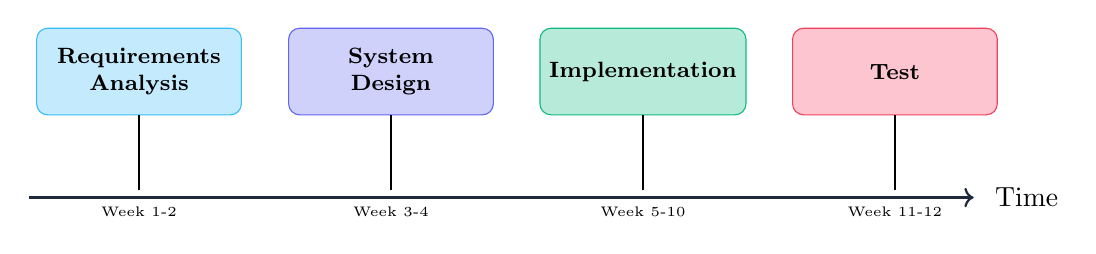
\begin{tikzpicture}[
    x=1cm, y=1cm,
    phase/.style={
        rectangle, rounded corners, draw,
        minimum width=2.6cm, minimum height=1.1cm,
        font=\footnotesize\bfseries, align=center
    }
]

    \coordinate (xReq) at (1.6,0);
    \coordinate (xDes) at (4.8,0);
    \coordinate (xImp) at (8.0,0);
    \coordinate (xTes) at (11.2,0);

    \draw[->, thick, darkbg] (0.2,0) -- (12.2,0);
    \node[anchor=west] at (12.35,0) {Time};

    \node[phase, fill=primary!30,   draw=primary]   (req)  at (1.6, 1.6) {Requirements\\Analysis};
    \node[phase, fill=secondary!30, draw=secondary] (des)  at (4.8, 1.6) {System\\Design};
    \node[phase, fill=success!30,   draw=success]   (impl) at (8.0, 1.6) {Implementation};
    \node[phase, fill=accent!30,    draw=accent]    (test) at (11.2,1.6) {Test};

    \draw[thick] (1.6,0.1) -- (req);
    \draw[thick] (4.8,0.1) -- (des);
    \draw[thick] (8.0,0.1) -- (impl);
    \draw[thick] (11.2,0.1) -- (test);

    \node[font=\tiny, below] at (1.6,0)  {Week 1-2};
    \node[font=\tiny, below] at (4.8,0)  {Week 3-4};
    \node[font=\tiny, below] at (8.0,0)  {Week 5-10};
    \node[font=\tiny, below] at (11.2,0) {Week 11-12};
\end{tikzpicture}
\end{center}
    
    \vspace{0.3cm}
    \begin{columns}[T]
        \column{0.5\textwidth}
        \textbf{Tools Used:}
        \begin{itemize}
            \item \faGitAlt\ Git + GitHub (Version Control)
            \item \faCode\ VS Code (Development)
            \item \faDatabase\ MySQL Workbench
        \end{itemize}
        \column{0.5\textwidth}
        \textbf{Collaboration:}
        \begin{itemize}
            \item Feature branches workflow
            \item Code reviews via Pull Requests
            \item Regular team meetings
            \item Shared documentation
        \end{itemize}
    \end{columns}
\end{frame}

% ============================================
% SLIDE 9: ARCHITECTURE
% ============================================
\section{System Architecture}
\begin{frame}{High-Level Architecture}
    \begin{center}
        \begin{tikzpicture}[scale=0.85, transform shape,
            box/.style={rectangle, rounded corners, draw, minimum width=3.5cm, minimum height=1.5cm, font=\bfseries, drop shadow, align=center},
            arrow/.style={-{Stealth}, thick}
        ]
            \node[box, fill=primary!20, draw=primary] (fe) at (0,0) {\faReact\ React Frontend\\(Vite + SPA)};
            \node[box, fill=success!20, draw=success] (be) at (5,0) {\faNodeJs\ Node.js Backend\\(Express API)};
            \node[box, fill=warning!20, draw=warning] (db) at (10,0) {\faDatabase\ MySQL Database\\(InnoDB)};

            \draw[arrow, <->] (fe) -- node[above, font=\tiny] {HTTP/JSON} node[below, font=\tiny] {REST API} (be);
            \draw[arrow, <->] (be) -- node[above, font=\tiny] {SQL} node[below, font=\tiny] {mysql2 driver} (db);
        \end{tikzpicture}
    \end{center}

    \vspace{0.3cm}
    \begin{columns}[T]
        \column{0.33\textwidth}
        \begin{block}{Frontend Stack}
            \scriptsize
            • React 18 + Hooks\\
            • React Router v6\\
            • TanStack Query\\
            • Axios HTTP Client\\
            • DOMPurify (XSS)
        \end{block}
        
        \column{0.33\textwidth}
        \begin{block}{Backend Stack}
            \scriptsize
            • Express.js 4.x\\
            • mysql2 (pooling)\\
            • bcryptjs (hashing)\\
            • Helmet (security)\\
            • express-rate-limit
        \end{block}
        
        \column{0.33\textwidth}
        \begin{block}{Database}
            \scriptsize
            • MySQL 8.0\\
            • 5 Tables\\
            • Foreign Keys\\
            • Indexes\\
            • Cascading deletes
        \end{block}
    \end{columns}
\end{frame}

% ============================================
% SLIDE 10: DATABASE
% ============================================
\begin{frame}{Database Schema (ER Diagram)}
    \begin{center}
    \resizebox{\textwidth}{!}{
        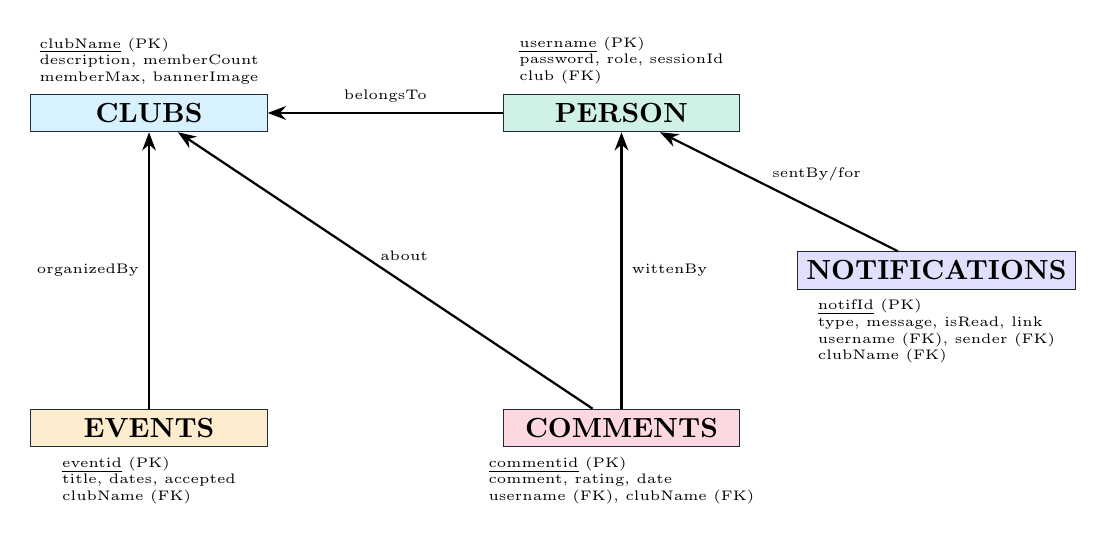
\begin{tikzpicture}[
            node distance=1cm,
            entity/.style={rectangle, draw=darkbg, fill=white, minimum width=3cm, font=\bfseries},
            attr/.style={font=\tiny, align=left}
        ]
            % CLUB
            \node[entity, fill=primary!20] (clubs) at (0,4) {CLUBS};
            \node[attr, above=0pt of clubs] {
                \underline{clubName} (PK)\\
                description, memberCount\\
                memberMax, bannerImage
            };

            % PERSON
            \node[entity, fill=success!20] (person) at (6,4) {PERSON};
            \node[attr, above=0pt of person] {
                \underline{username} (PK)\\
                password, role, sessionId\\
                club (FK)
            };

            % EVENTS
            \node[entity, fill=warning!20] (events) at (0,0) {EVENTS};
            \node[attr, below=0pt of events] {
                \underline{eventid} (PK)\\
                title, dates, accepted\\
                clubName (FK)
            };

            % COMMENTS
            \node[entity, fill=accent!20] (comments) at (6,0) {COMMENTS};
            \node[attr, below=0pt of comments] {
                \underline{commentid} (PK)\\
                comment, rating, date\\
                username (FK), clubName (FK)
            };

            % NOTIFICATIONS
            \node[entity, fill=secondary!20] (notif) at (10,2) {NOTIFICATIONS};
             \node[attr, below=0pt of notif] {
                \underline{notifId} (PK)\\
                type, message, isRead, link\\
                username (FK), sender (FK)\\
                clubName (FK)
            };

            % Relationships
            \draw[thick, -{Stealth}] (person) -- node[above, font=\tiny] {belongsTo} (clubs);
            \draw[thick, -{Stealth}] (events) -- node[left, font=\tiny] {organizedBy} (clubs);
            \draw[thick, -{Stealth}] (comments) -- node[right, font=\tiny] {wittenBy} (person);
            \draw[thick, -{Stealth}] (notif) -- node[above, font=\tiny]
            {\quad \quad \quad \quad sentBy/for} (person);
            \draw[thick, -{Stealth}] (comments) -- node[above, font=\tiny]
            {\quad \quad about} (clubs);
        \end{tikzpicture}
    }
    \end{center}
\end{frame}

% ============================================
% SLIDE 11: API
% ============================================
\begin{frame}{API Endpoints Structure}
    \begin{columns}[T]
        \column{0.5\textwidth}
        \textbf{Auth \& Clubs}
        \tiny
        \begin{tabular}{ll}
            \toprule
            \textbf{Method} & \textbf{Endpoint} \\
            \midrule
            \rowcolor{success!10} POST & /login \\
            \rowcolor{success!10} POST & /logout \\
            GET & /clubs \\
            POST & /createClub (Auth: STU) \\
            DELETE & /clubs/:name (Auth: CL) \\
            \bottomrule
        \end{tabular}
        
        \vspace{0.2cm}
        \textbf{Events}
        \tiny
        \begin{tabular}{ll}
            \toprule
            \textbf{Method} & \textbf{Endpoint} \\
            \midrule
            GET & /events \\
            POST & /createEvent (Auth: CL/VP) \\
            PUT & /event/:id (Auth: CL) \\
            \bottomrule
        \end{tabular}

        \column{0.5\textwidth}
        \textbf{Member Management}
        \tiny
        \begin{tabular}{ll}
            \toprule
            \textbf{Method} & \textbf{Endpoint} \\
            \midrule
            PUT & /joinClubs/:club \\
            PUT & /accept/:user (Auth: CL/VP) \\
            PUT & /expell/:user (Auth: CL/VP) \\
            PUT & /promote/:user (Auth: CL) \\
            DELETE & /quitClub \\
            \bottomrule
        \end{tabular}
        
        \vspace{0.2cm}
        \textbf{Social}
        \tiny
        \begin{tabular}{ll}
            \toprule
            \textbf{Method} & \textbf{Endpoint} \\
            \midrule
            GET & /notifications \\
            POST & /comment \\
            DELETE & /comment/:id \\
            \bottomrule
        \end{tabular}
    \end{columns}
    \vspace{0.3cm}
    \begin{center}
        \footnotesize \textit{All protected endpoints require \texttt{x-username} and \texttt{x-session-id} headers}
    \end{center}
\end{frame}

% ============================================
% SLIDE 12: FRONTEND STRUCTURE
% ============================================
\begin{frame}{Frontend Component Structure}
    \begin{center}
        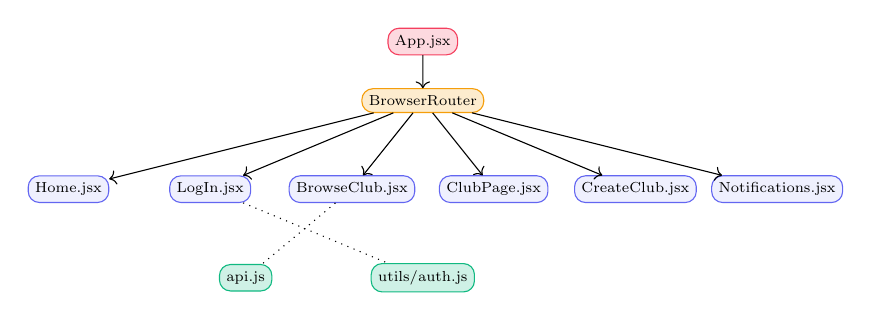
\begin{tikzpicture}[scale=0.75, transform shape,
            comp/.style={rectangle, draw=primary, fill=primary!10, rounded corners, font=\scriptsize},
            page/.style={rectangle, draw=secondary, fill=secondary!10, rounded corners, font=\scriptsize}
        ]
            \node[comp, fill=accent!20, draw=accent] (app) at (6,4) {App.jsx};
            \node[comp, fill=warning!20, draw=warning] (router) at (6,3) {BrowserRouter};
            
            \node[page] (home) at (0,1.5) {Home.jsx};
            \node[page] (login) at (2.4,1.5) {LogIn.jsx};
            \node[page] (browse) at (4.8,1.5) {BrowseClub.jsx};
            \node[page] (club) at (7.2,1.5) {ClubPage.jsx};
            \node[page] (create) at (9.6,1.5) {CreateClub.jsx};
            \node[page] (notif) at (12,1.5) {Notifications.jsx};

            \draw[->] (app) -- (router);
            \foreach \x in {home, login, browse, club, create, notif}
                \draw[->] (router) -- (\x);

            \node[comp, fill=success!20, draw=success] (api) at (3,0) {api.js};
            \node[comp, fill=success!20, draw=success] (auth) at (6,0) {utils/auth.js};
            
            \draw[dotted] (login) -- (auth);
            \draw[dotted] (browse) -- (api);
        \end{tikzpicture}
    \end{center}
    
    \begin{columns}[T]
        \column{0.5\textwidth}
        \textbf{Key Libraries:}
        \begin{itemize}
            \item TanStack Query (Data Fetching)
            \item React Router (Navigation)
            \item DOMPurify (XSS Protection)
        \end{itemize}
        \column{0.5\textwidth}
        \textbf{State Management:}
        \begin{itemize}
            \item Local state (useState)
            \item Session in localStorage
            \item Server state via React Query
        \end{itemize}
    \end{columns}
\end{frame}

% ============================================
% SLIDE 13: AUTHENTICATION & SECURITY (NEW)
% ============================================
\begin{frame}{Authentication \& Security}
\small
\begin{columns}[T]
    \column{0.56\textwidth}
    \textbf{\faKey\ Authentication Flow}
    \begin{itemize}
        \item \textbf{Signup/Login}: bcrypt password hashing + verification
        \item Backend issues a \textbf{sessionId (UUID)} stored in \texttt{person.sessionId}
        \item Frontend stores session in \texttt{localStorage} (\texttt{sca\_session})
        \item Axios sends \texttt{x-username} and \texttt{x-session-id} on every request
        \item Middleware \texttt{requireAuth} validates the session and attaches \texttt{req.user}
    \end{itemize}

    \column{0.44\textwidth}
    \textbf{\faShieldAlt\ Security Controls}
    \begin{itemize}
        \item \textbf{RBAC}: \texttt{requireRoles} (CL/VP/CM/STU) + club ownership checks
        \item \textbf{XSS protection}: DOMPurify sanitization for HTML club descriptions
        \item \textbf{API hardening}: Helmet headers + rate limiting + JSON size limit
        \item \textbf{SQL safety}: parameterized queries (\texttt{?}) + whitelisted sorting
    \end{itemize}
\end{columns}

\vspace{0.2cm}
\begin{center}
\scriptsize \textit{Invalid sessions return 401 and the client clears \texttt{sca\_session} and redirects to Login.}
\end{center}
\end{frame}

% ============================================
% SLIDE 14: DESIGN PATTERNS
% ============================================
\section{Design Decisions}
\begin{frame}{Design Decisions \& Patterns}
    \begin{columns}[T]
        \column{0.5\textwidth}
        \textbf{Technology Choices:}
        \begin{itemize}
            \item \textbf{React+Vite:} Reusability, Virtual DOM, HMR.
            \item \textbf{Node+Express:} Fullstack JS, Middleware ecosystem.
            \item \textbf{MySQL:} Relational data, ACID, Foreign Keys.
        \end{itemize}
        
        \column{0.5\textwidth}
        \textbf{Design Patterns Used:}
        \begin{itemize}
            \item \textbf{Middleware:} Auth, Rate limiting.
            \item \textbf{Repository:} DB query abstraction.
            \item \textbf{Observer:} Notification system.
            \item \textbf{Singleton:} DB connection pool.
        \end{itemize}
        
        \vspace{0.2cm}
        \begin{block}{Architecture}
            3-Tier Architecture + RESTful API design.
        \end{block}
    \end{columns}
\end{frame}

% ============================================
% SLIDE 15: RETROSPECTIVE
% ============================================
\section{Retrospective}
\begin{frame}{Retrospective}
    \begin{columns}[T]
        \column{0.5\textwidth}
        \begin{block}{\faCheck\ What Worked Well}
            \begin{itemize}
                \item Clean separation of frontend/backend
                \item React Query simplified data management
                \item Well-designed DB schema upfront
                \item Git workflow prevented conflicts
            \end{itemize}
        \end{block}
        
        \column{0.5\textwidth}
        \begin{alertblock}{\faExclamationTriangle\ Challenges}
            \begin{itemize}
                \item Session management across reloads
                \item Role-based UI rendering
                \item Async state synchronization
                \item Initial CORS configuration
            \end{itemize}
        \end{alertblock}
    \end{columns}
    
    \vspace{0.3cm}
    \begin{center}
        \textbf{Lesson Learned:} Upfront design saves debugging time.
    \end{center}
\end{frame}

% ============================================
% SLIDE 16: FUTURE IMPROVEMENTS
% ============================================
\begin{frame}{Future Improvements}
    \begin{center}
        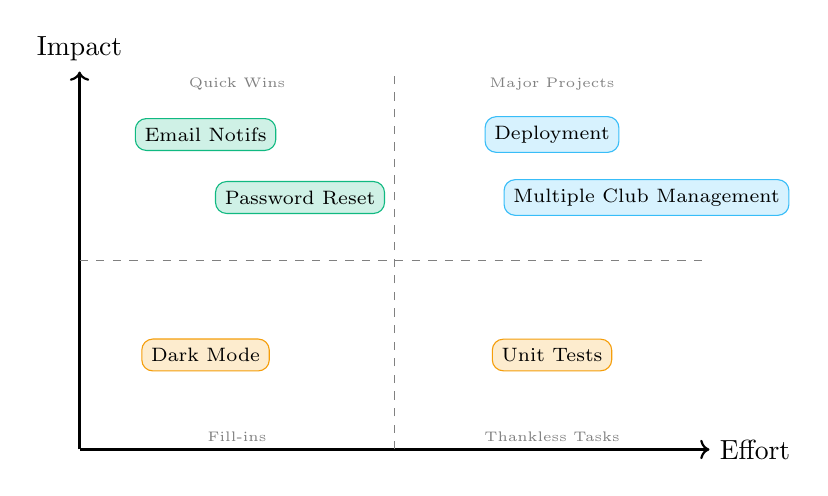
\begin{tikzpicture}[scale=0.8]
            % Axes
            \draw[->, thick] (0,0) -- (10,0) node[right] {Effort};
            \draw[->, thick] (0,0) -- (0,6) node[above] {Impact};
            
            % Quadrants
            \draw[dashed, gray] (5,0) -- (5,6);
            \draw[dashed, gray] (0,3) -- (10,3);
            
            % Labels
            \node[gray, font=\tiny] at (2.5, 5.8) {Quick Wins};
            \node[gray, font=\tiny] at (7.5, 5.8) {Major Projects};
            \node[gray, font=\tiny] at (2.5, 0.2) {Fill-ins};
            \node[gray, font=\tiny] at (7.5, 0.2) {Thankless Tasks};
            
            % Items
            \node[rectangle, draw=success, fill=success!20, rounded corners, font=\scriptsize] at (2,5) {Email Notifs};
            \node[rectangle, draw=success, fill=success!20, rounded corners, font=\scriptsize] at (3.5,4) {Password Reset};
            
            \node[rectangle, draw=primary, fill=primary!20, rounded corners, font=\scriptsize] at (7.5,5) {Deployment};
            \node[rectangle, draw=primary, fill=primary!20, rounded corners, font=\scriptsize] at (9,4) {Multiple Club Management};

            \node[rectangle, draw=warning, fill=warning!20, rounded corners, font=\scriptsize] at (2,1.5) {Dark Mode};
            \node[rectangle, draw=warning, fill=warning!20, rounded corners, font=\scriptsize] at (7.5,1.5) {Unit Tests};
        \end{tikzpicture}
    \end{center}
\end{frame}

% ============================================
% SLIDE 17: CONTRIBUTIONS
% ============================================
\section{Team Contributions}
\begin{frame}{Individual Contributions}
    \begin{columns}[T]
        \column{0.5\textwidth}
        \textbf{\faUser\ Francesco Bolner}
        \begin{itemize}
            \item Database Schema Design
            \item Notifications System
        \end{itemize}
        
        \vspace{0.2cm}
        \textbf{\faUser\ Ayoub Merdan}
        \begin{itemize}
            \item Authentication System
            \item Security Implementation
        \end{itemize}

        \vspace{0.2cm}
        \textbf{\faUser\ Martin Ushilov}
        \begin{itemize}
            \item Backend API Endpoints
            \item Testing \& Documentation
        \end{itemize}

        \column{0.5\textwidth}
        \textbf{\faUser\ Georgi Bozhkov}
        \begin{itemize}
            \item Frontend Components
            \item React Query Integration
        \end{itemize}
        
        \vspace{0.2cm}
        \textbf{\faUser\ Samuele Fumagalli}
        \begin{itemize}
            \item UI/UX Design
            \item CSS Styling
        \end{itemize}
    \end{columns}
\end{frame}

% ============================================
% SLIDE 18: LIVE DEMO
% ============================================
\section{Live Demo (MVP)}
\begin{frame}{Live Demonstration}
    \begin{center}
        \Huge\faLaptopCode\\[0.3cm]
        \large\textbf{MVP Live Demo}\\[0.2cm]
        \normalsize\textit{Switch to Browser for Live Walkthrough}
    \end{center}
    
    \vspace{0.5cm}
    \begin{columns}[T]
        \column{0.5\textwidth}
        \textbf{Student Scenarios:}
        \begin{enumerate}
            \item \faSignInAlt\ Login as Student
            \item \faSearch\ Browse \& Search Clubs
            \item \faEye\ View Club Details
            \item \faUserPlus\ Request to Join Club
            \item \faCommentDots\ Post Comment with Rating
        \end{enumerate}
        
        \column{0.5\textwidth}
        \textbf{Admin/Leader Scenarios:}
        \begin{enumerate}
            \item \faSignInAlt\ Login as Club Leader
            \item \faCalendarPlus\ Create New Event
            \item \faUserCheck\ Approve Member Request
            \item \faUserTie\ Promote Member to VP
            \item \faBell\ View Notifications
        \end{enumerate}
    \end{columns}
\end{frame}

% ============================================
% SLIDE 19: QUESTIONS
% ============================================
\section{Q\&A}
\begin{frame}
\begin{center}
    \Huge \faQuestionCircle\\[0.5cm]
    \textbf{Questions?}\\[1cm]
    \normalsize
    Thank you for your attention!\\[0.3cm]
    \faGithub\ \href{https://github.com/gbozhkov/Software-Engineering-1-Project}{github.com/gbozhkov/Software-Engineering-1-Project}
\end{center}
\end{frame}

\end{document}

